\section{Sampling \& Simplifications}
    \begin{frame}[t]
        \frametitle{Probability Calculations}
        
        \vspace{-0.6cm}

        \begin{columns}[t]
            \column{0.4\textwidth}
                \begin{itemize}
                    \item Full probability still requires normalization \pause
                    \item Switch to the Metropolis \emph{Hastings} algorithm
                    \begin{itemize}
                        \item Non-exponential number of samples \pause
                        \item Depends only on a transition probability
                        \item Does not need normalization because it cancels
                    \end{itemize}
                \end{itemize}
    
            \onslide
            \column{0.4\textwidth}
                \vspace{0.0cm}
                \pause[3]
                \makebox[\textwidth][c]{
                    \includegraphics[width=1.3\textwidth,page=2]{main-content/simplifications/mc-sampling.pdf}
                }
    
        \end{columns}

        \pause[2]
        \vspace{0.15cm}
        \makebox[\textwidth][c]{
            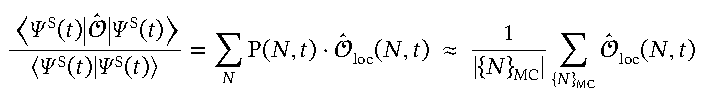
\includegraphics[width=0.80\textwidth,page=1]{main-content/simplifications/mc-sampling.pdf}
        }

        % notes 
        \onslide % on all slides of frame
        \note[item] {
            Normalization requires knowing exponential amount of states and we need to sample an exponential amount to get all
        }
    \end{frame}

    \begin{frame}[t]
        \frametitle{Analytical Simplifications}
        
        \begin{itemize}
            \item Choose a helpful initial state
        \end{itemize}
    
        \pause
        \vspace{-0.35cm}
        \makebox[\textwidth][c]{
            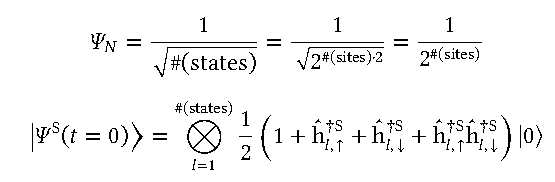
\includegraphics[width=0.60\textwidth,page=1]{main-content/simplifications/analytical-simplification-example.pdf}
        }

        \vspace{-0.1cm}
        \begin{itemize}
            \item Now \emph{almost all} terms cancel in \emph{differences} of the effective Hamiltonian \pause
            \begin{itemize}
                \item Exemplary for single flip on base energy term
            \end{itemize} 
        \end{itemize}

        \vspace{-0.15cm}
        \makebox[\textwidth][c]{
            \includegraphics[width=0.62\textwidth,page=2]{main-content/simplifications/analytical-simplification-example.pdf}
        }

        % notes 
        \onslide % on all slides of frame
        \note[item] {
            TODO
        }
    \end{frame}
